\documentclass[a4paper]{article}
\usepackage[dutch]{babel}
\usepackage{geometry}
\usepackage[utf8]{inputenc}
\usepackage{hyperref}
\usepackage{listings}
\usepackage{graphicx}
\usepackage[x11names, rgb, html]{xcolor}

% dimensions
\geometry{left=3cm, top=3cm, right=3cm, bottom=3cm}

% font
\usepackage{DejaVuSans}
\renewcommand*\familydefault{\sfdefault}
\usepackage[T1]{fontenc}

% hyperlinks
\hypersetup{%
  colorlinks=true,
  linkcolor=blue,
  urlcolor=cyan,
}

% image
\graphicspath{{img/}}

% lists
\providecommand{\tightlist}{%
\setlength{\itemsep}{0pt}\setlength{\parskip}{0pt}}

% preamble
\title{Experiments}
\author{Tim Visée \& Nathan Bakhuijzen}
\date{October 2018}

\begin{document}

  \pagenumbering{gobble}
  \maketitle
  \begin{figure}[h]
    \centering
    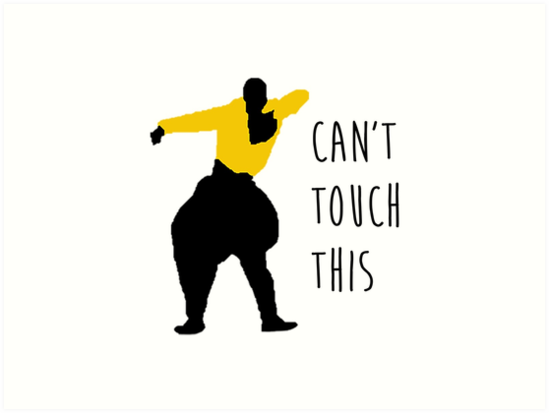
\includegraphics[width=\linewidth]{cant-touch-this}
  \end{figure}
  \clearpage

  \section*{Preface}
  In this document, we will go through some experiments we've conducted for the
  platform we have built during the research minor KB-80. For each experiment
  we've written a new section describing what it is about, how we conduct the
  experiment and what our findings are. The general idea of conducing these
  experiments is to assert whether the current platform is \emph{usable} for
  the purpose we had originally in mind, namely controlling a generic computer.

  Although we've tested the platform quite thoroughly while building it, these
  experiments are conducted on the final version of the platform we've worked on
  with properly detected experiments and findings. With this we'll attempt to
  also answer some seemingly obvious thoughts.

  \paragraph{}
  The last part of the document goes over some ideas we came up with when
  working on on the project, and when conducting these experiments. These
  ideas may be implemented by others that continue the work on this project.

  \paragraph{}
  You may of course conduct similar experiments as we've described along with
  reading this document. Make sure you read the \emph{Manual} on how to install
  and use the product.

  \clearpage

  \section*{Accuracy \& Reliability}
  The accuracy and reliability of the gesture recognition is crucial to the
  succes of the platform. If it proves to be insufficient, then the platform is
  obsolete. No one will use it and time spent developing it will be wasted. If
  it is accurate and reliable however, then it may prove useful. It may be used
  to conduct further research, and can be developed further.

  To test our platform, we came up with a list of predefined gestures. These
  gestures are programmed/\emph{hard-coded} into the platform. This means that the predefined
  gesture is not jittery to begin with, as could be the case with recorded
  gestures. This is our list of predefined gestures:
  \begin{itemize}
    \tightlist
    \item Straight line
    \item Circle clockwise
    \item Circle counter-clockwise
    \item Big circle clockwise
    \item Big circle counter-clockwise
    \item Triangle clockwise
    \item Triangle counter-clockwise
    \item Mini square clockwise
    \item Square clockwise
    \item Square counter-clockwise
  \end{itemize}

  When we tested these gestures ourselves, we found that most of them work very
  well. The \textit{straight line} till the \textit{Big circle counter-clockwise}
  all work great. This is because the gestures have continual change. That means
  that the hand or fingers always move in a different direction than before.

  Gestures like the \textit{triangle} and \textit{square} work not as good as
  expected. These gestures have a tendency to not get recognized if the change
  in the direction is too great or after a long consistent pattern. This is
  because the gesture programmed into the platform has a specific check for
  change in directions. If the gesture deviates too much, the entire gesture
  will not be recognized. This is unfortunate, because that means that the
  gesture can be performed almost perfectly, only to be messed up at the end,
  resulting in a failure to recognize the gesture.

  % TODO: explain clearly that this is wat we figured because of our findings above
  We also found out that sharp corners and long gestures don't work very well.
  Improvement of the gesture recognition could change this in the future.

  This means that our gesture recognition can definitely be improved. Comparing
  gestures based on certain changes on a predefined distance is not effective.
  This means that the recognition has to be improved in order to implement even
  more complicated gestures.

  Some properties of the current gesture recognition can be altered in the \textit{config.rs}
  file. By including a larger amount of points in a match group/scope, failure to recognize a
  gesture will be lower. This is because there will be more points, and more
  room for deviation from the predefined gesture. Following this approach would
  allow more false positives though.

  \clearpage

  \section*{Gesture variety}
  For building a proper gesture based system, we think it is important to
  support as many gestures as possible. If you're binding gestures to actions on
  a computer, you probably want to do as much different things as possible with
  a little difficult gestures as possible. We'll now attempt to define what
  variety of gestures is possible with our current implementation.

  \paragraph{}
  The platform currently has support for tracking gestures based on movements
  with the tip of the index finger. This already limits the number of gesture
  possibilities quite severely. You basically need to use your finger as a pen
  or wand to literally draw a shape.

  In addition, recorded sensor data is currently being processed into a 2D
  representation. This means that it is currently not possible to define 3D
  aware gestures.

  \paragraph{}
  As shown in the previous experiment, large gestures or gestures with sharp
  corners don't work to well yet with the current algorithm without tweaks.

  \subsection*{Supported}
  When only defining basic gestures, we could think of the following gesture
  types:

  \begin{itemize}
    \tightlist
    \item Circle
    \item Line
    \item Square
    \item Rectangle, in various shapes
    \item Triangle
    \item Simple/distinct numbers: 2, 3, 6, 7
    \item Simple/distinct letters: C, D, J\dots
    \item \dots
  \end{itemize}

  Each figure can have some variations:
  \begin{itemize}
    \tightlist
    \item Various figure scales, larger and smaller variants
    \item Use both clockwise and counter-clockwise variants
    \item Scale in one dimension, use an oval instead of a circle
  \end{itemize}

  The list is limited, and some variations might collide resulting in false
  positives. Implementing 10 different gestures is however easily doable, as the
  built-in list of gestures does confirm. The question of whether the variety is
  good enough highly depends on the use case for the product.
  % TODO: should have a better story here

  \subsection*{TODO: Computer control}
  % TODO: - do we think the current system supports enough to control a computer
  Now, the initial goal of the platform was to develop a platform that would be
  able to fully control a computer using only gestures. We currently don't think
  that that is possible, let alone viable. This is a list of problems that would
  have to be resolved in order for the platform to become viable:

  \begin{itemize}
    \tightlist
    \item Not all gestures are recognized properly.
    \item Gestures do not support multiple fingers
    \item The predefined gestures are limited
    \item New recorded gestures could be jittery, resulting in a low recognition
      rate
    \item Execution of computer actions would probably slower than using a
      keyboard and mouse
  \end{itemize}

  We know that this is a lot to ask for, but if we would be able to solve these
  problems we could have built a revolutionary new platform.

  \subsection*{Improve}
  To improve the results of this test, we believe that additional features need
  to be developed in the platform which does take some time. Think of supporting
  gestures consisting of multiple fingers or even hands, or supporting 3D
  gestures. If multiple fingers are combined in gestures, then it could mean a
  plethora of new possibilities. Improvements would mostly consist of software improvements rather
  than needing to have improved hardware. Think of changes in the algorithm and
  processing logic to allow more advanced figures. We'll go over ideas for
  improvement in the \emph{Ideas} section, the last section in this document.

  \clearpage

  \section*{Visual feedback}
  An interesting aspect for using our platform is visual feedback, and what the
  effect of using it is on users using our platform. With visual feedback, a
  user would be able to see on a computer screen how the computer (or rather;
  sensor) recognizes his hand(s) and/or gestures. The general idea for this test
  is that showing visual feedback might improve accuracy, as users could adapt
  the gesture they're performing on what they see the computer recognizes.
  The sensor isn't super accurate all of the time, or users might go outside the
  view of the sensor. The visual feedback would immediately show this.

  \subsection*{Visualizers}
  Two visualizers are available. The first one is part of the LeapMotion
  software package, and is a 3D visualizer that can be started from the
  LeapMotion control panel. This visualizer shows a 3D representation of
  recognized hands above the LeapMotion sensor inside the bounding box of the
  sensor. Joints are visible in the hand, although our software only uses the
  position of the index finger tip at this moment.

  The second visualizer is the one we've implemented. It is show on the web
  interface that can be opened after starting the software. This visualizer is
  quite different, not only in aesthetics, but also in what it shows. Our
  visualizer is 2D and shows the data that has been processed by our software.
  The \emph{Manual} explains how we are processing the data, and that we're
  mapping 3D points from the sensor in traces of rotational data. This is what
  is rendered in our visualizer, and is essentially what is used for gesture
  detection. This is therefore \emph{closest to reality}, where \emph{reality}
  consists of user defined gestures in our software and the recognition system.
  If gestures show up correctly in this visualizer, the software should
  recognize them correctly. This same visualizer is used for recording and
  trimming new gestures.

  \subsection*{Findings}
  For this test we've tried a lot of different gestures, in a lot of different
  positions. Here are some of our statements on our findings:

  \begin{itemize}
    \item Drawing circles isn't a problem. The only thing a visualizer might
      help for is to see whether you're performing the gestures within the
      view of the sensor, and to see whether your hand is properly recognized.
    \item Without visual feedback attempting to draw squares, can easily result
      in drawing rectangles, especially when focussing on the screen instead of
      looking at your hand. Having the 2D web visualizer helps greatly as you
      can see whether you're drawing a square properly.
    \item The 3D visualizer is easier to understand, although the data shown in
      the 2D visualizer is more consistent. This, in the sense that using the 2D
      visualizer to guide you to perfectly draw a gesture works better and
      produces more accurate results than using the 3D visualizer.
    \item Either visualizer is useful to see whether the sensor is
      jittering, causing detection failures.
    \item Properly drawing a gesture with the other hand a gesture was
      recorded with is virtually impossible without a visualizer, except for
      shapes that are really simple.
    \item The 2D web visualizer gives a better sense of how big a user is
      drawing a gesture. Allowing the user to be more accurate.
    \item The 2D web visualizer is useful to figure out why a false positive may
      have been detected as it clearly shows the shape that is used for
      recognition.
  \end{itemize}

  \subsection*{Conclusion}
  Based on these statements we can conclude that using a visualizer is a good
  idea, as it does seem to improve results for most gestures. There are gestures
  however that don't really benefit from using a visualizer. Such gestures can
  be used in a situation where a visualizer isn't preferred as it would use up
  screen real estate.

  The accuracy of a user drawing a gesture correctly might improve the more the
  user uses the system. We haven't tested this.

  \paragraph{}
  None of the visualizers notify the user if a drawn gesture is similar to a
  user defined gesture (but is not a match). Imagine that you're drawing a
  circle, but too large for it to be detected. The visualizers don't show that
  your circle is too large. This might be something to improve on.

  \paragraph{}
  Note that we, the developers of the platform, have conducted this test. Other
  users that don't understand the internals of the system might experience this
  different. The second visualizer in the web interface shows processed data,
  this might look weird and unintuitive for other users.

  \clearpage

  \section*{TODO: Recognition consistency}
  % TODO: we aren't performing gesture many times to improve accuracy
  It is important that all gestures are successfully performed and can be recognized
  multiple times. This is because recognizing gestures can be error-prone. By
  performing gestures often, the risk of it recognizing a gesture incorrectly
  decreases dramatically.

  \clearpage

  \section*{Detection speed}
  Another important aspect of the gesture recognition system is the speed, or
  rather, the delay for detecting a performed gesture. To avoid confusion, we've
  decided to define the term delay as follows: \textit{The time it takes for the
    platform to show the name of the correct gesture in the console, after a
    gesture has been completely performed above the sensor}.

  \subsection*{Counting frames}
  Since it can be tricky to accurately measure the time difference between an
  invocation and an action, we've decided to record 20 invocations.
  With the resulting footage, we'll be able to count delay in
  frames, with precision accurately enough for our use case. The gesture that we
  choose was the square, as is has quite distinctive corners.

  \subsection*{Results}
  After performing the our own tests it was quite clear that delay varies
  greatly. The \emph{delay} varied from about 5 to 11 frames. With a speed of 60
  frames per second, each frame is about 17 milliseconds. This defines a delay
  varying between 85 to 187 milliseconds. There were two outliers with a delay
  of 16 to 22 frames which translate to about 270 and 370 milliseconds.

  We believe the varying difference has to do with the accuracy of detecting the
  gesture itself. Imagine you are drawing a perfect square gesture (perfect
  relative to the square gesture you might have previously recorded) above the
  sensor, the gesture will be recognized quicker before even fully completing
  the gesture, as compared to a square motion that differs slightly. Because
  it's virtually impossible to perform the gesture in exactly the same way every
  iteration, a difference in detection is indeed expected.

  Note that our method of testing latency is still quite simplistic. It doesn't
  take computer and screen delay into account. Nor does it test what the latency
  of the used sensor itself is. Our test strictly focusses on the delay between
  performing the gesture and seeing visual feedback. We performed the test with
  the visualizer enabled, which was visible on the material we recorded. What's
  interesting is that it looks like the gesture is instantly (meaning; within
  the same frame) recognized as the last sampled point of a gesture shows up on
  the visualizer. This would suggest that the actual latency for detection on
  the processed data is faster than 17 milliseconds. This is of course not very
  scientific, but we feel it's an awesome result non the less.

  What is important though, is how responsive the detection feels. During these
  tests, the detection (strictly speaking about detection speed) felt snappy even
  during the case of those outliers. The cool thing is that after you've
  performed a gesture you don't have to wait for a detection notification before
  the next gesture can be performed, that helps quite a lot for it to feel
  responsive to our opinion when when repeatedly experimenting with the sensor.

  The platform doesn't support binding
  generic actions to gestures to control a computer yet. And until that is
  tested, it's hard to say whether we'd feel the same when controlling a
  computer with these gestures. We mention this idea of binding actions later in
  this report in the \emph{Ideas} section.

  \clearpage

  \section*{Ideas}
  During the project, and during the experiments we've conducted we came up with
  quite a few ideas. Some of them are things we'd wanted to implement but didn't
  have the time for it due to time constraints. Other ideas originate from
  test results we've collected.
  Here follow a few of them:

  \subsection*{Multiple fingers}
  The current system only has support for gestures consisting of a single trace,
  being the trace drawn by the index finger of a hand. The first logical
  expansion would of course be to support gestures having motions with 5
  fingers. Sadly, due to time constraints, we couldn't implement this.
  This could be a great opportunity to improve the complexity and depth of the platform.

  Our guess is that implementing this isn't too hard when using the same
  detection system as our current platform. The implementation might be as easy
  as extending our \verb_Hand_ structure (in code) to contain 5 traces, instead
  of just 1. This might be cool to experiment with for other groups taking a
  look at this project.

  \subsubsection*{Not just finger tips}
  With the extension described above, the system would still only be tracking
  finger tips. The sensor we're currently using is able to report the position
  of all joints in a hand, including the center of each bone and the center of
  the hand palm. This is easily visible in the 3D visualizer that is provided
  with the LeapMotion software package. The \verb_leap-rs_ wrapper that is
  currently used doesn't have an interface to obtain this information yet,
  but this could be implemented without too much effort.

  The same might be true for this implementation, just tracking the trace for
  every joint might be enough. We're of course not sure, that's something cool
  to test out.

  \subsection*{3D detection}
  Although we intended to support it at first, 3D gesture detection would be an
  awesome improvement. The current system uses 2D rotational data to represent
  user motions. Simply said; because of processing data to this format, the
  third dimension is lost. We found it difficult to reliably transform a 3D
  curve into 2D rotation data, and wanted to get the 2D system working first.

  Of course, motions in 3D space are transformed into data our platform uses.
  During this process the depth (Z-axis) is lost though. Drawing a circle
  sideways would be detected as moving up and down on a straight line. In this
  system, you might imagine drawing on a virtual plane on the X and Y axis.
  Supporting the Z-axis as well for a 3rd dimension would open up a lot of new
  possibilities for drawing gestures in different orientations and would support
  much more complex gestures.

  \subsection*{Bindable actions}
  Our idea was to allow users to bind custom actions to recorded gesture
  templates quite early in the project. This would allow a user to configure the
  platform to control their computer in a generic way. The implementation can be
  as simple as binding mouse (and scroll weel) actions, keys and system commands.

  Such an implementation would immediately make the project much more viable for
  use by others (given that it would work properly). This also opens new
  research questions such as; can gestures be complex enough to support enough
  gestures for controlling a generic computer?

  \paragraph{}
  This idea was also the segway to research on how usable a gesture detection
  system is for use in medical \& sterile environments. Imagine doctors not
  having to touch a röntgen machine to swipe between pictures, by using
  touchless hand gestures instead. The implementation of bindable actions
  should make quite clear whether such a system is usable and reliable.

  \subsection*{Multiple sensors}
  An awesome extension would be to use and combine multiple sensors in the
  platform, instead of using a single LeapMotion sensor. The obvious choice
  would be to use a second LeapMotion sensor to combine data of the two. This
  could be used to filter jitter, and to fallback if the view for one sensor os
  occluded.

  This is one of the first things we looked into during the project. Sadly, it
  became apparent that the LeapMotion SDK doesn't support connecting multiple
  sensors, even though the provided library would suggest otherwise as there are
  functions available to obtain a list of connected sensors.
  \href{https://forums.leapmotion.com/t/multiple-leap-motion-support/770}{This}
  forum thread is about this topic, in which users are asking for support to use
  multiple sensors. In this thread, LeapMotion developers have said this is not
  possible.

  \paragraph{}
  It would be fun to use a different computer, or possible a virtual machine
  with a virtual USB controller to support connecting another sensor.
  The data from this sensor would then need to be
  transmitted to the platform to collect the sensor data. This is however
  outside the scope of our project, and is a challenge to properly implement on it's own.

  \paragraph{}
  Another option is to implement support for other kinds of sensors, such as the
  XBox Kinect, or something different. Our platform would than need to provide
  the proper abstractions to aggregate the data from different kinds of sensors
  into something the platform could use.

\end{document}
